\chapter{Instrukcja wdrożeniowa}
Pliki źródłowe projektu zostały umieszczone w zdalnym repozytorium kodu na stonie github. 
Link do repozytorium: \url{https://github.com/Quarol/Praca-inzynierska.git}

Użytą wersją języka Python jest Python 3.12.4. Aby wykorzystać zaprojektowany system, należy ją zainstalować.

Repozytorium składa się z dwóch plików wykonywalnych (\emph{main.py}, \emph{install\_requirements.py}) oraz dwóch folderów -- \emph{assets} oraz \emph{detector}. Struktura pokazana na ryskunku \ref{fig:repo}.
Folder \emph{assets} zawiera plik dźwiękowy służący jako alarm w systemie. Folder \emph{detector} zawiera wsysztkie pliki źródłowe z opisanymi komponentami systemu.
Plik \emph{install\_requirements.py} to skrypt służący do instalacji wszystkich wykorzystanych modułów języka Python w użytych wersjach.
Plik \emph{main.py} jest to plik uruchamiający aplikację.

W celu instalacji modułów, a następnie uruchomieniu programu należy najpierw uruchomić plik \emph{install\_requirements.py}, a następnie \emph{main.py}. Pliki można uruchomić korzystając ze środowiska programistycznego lub poprzez komendy w terminalu. Komendy mogą różnić się w zależności od systemu operacyjnego oraz sposobu instalacji Pythona. W systemie windows zazwyczaj używa się komendy \emph{python}, przedstawionej na listingu \ref{lst:python_d}, zaś w systemie linux -- \emph{python3} (listing \ref{lst:python3}).

\begin{lstlisting}[caption={Komendy do instalacji modułów oraz uruchomienia aplikacji nr 1.}, label={lst:python_d}]
python install_requirements.py
python main.py
\end{lstlisting}

\begin{lstlisting}[caption={Komendy do instalacji modułów oraz uruchomienia aplikacji nr 2.}, label={lst:python3}]
python3 install_requirements.py
python3 main.py
\end{lstlisting}

\begin{figure}[H]
    \centering
    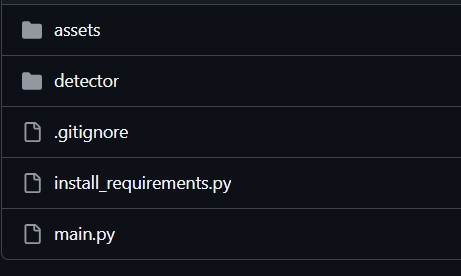
\includegraphics[width=0.55\linewidth]{_repo.jpg}
    \caption{Struktura repozytorium.}
    \label{fig:repo}
\end{figure}


